\documentclass[11pt,a4paper,]{article}
\usepackage{lmodern}

\usepackage{amssymb,amsmath}
\usepackage{ifxetex,ifluatex}
\usepackage{fixltx2e} % provides \textsubscript
\ifnum 0\ifxetex 1\fi\ifluatex 1\fi=0 % if pdftex
  \usepackage[T1]{fontenc}
  \usepackage[utf8]{inputenc}
\else % if luatex or xelatex
  \usepackage{unicode-math}
  \defaultfontfeatures{Ligatures=TeX,Scale=MatchLowercase}
\fi
% use upquote if available, for straight quotes in verbatim environments
\IfFileExists{upquote.sty}{\usepackage{upquote}}{}
% use microtype if available
\IfFileExists{microtype.sty}{%
\usepackage[]{microtype}
\UseMicrotypeSet[protrusion]{basicmath} % disable protrusion for tt fonts
}{}
\PassOptionsToPackage{hyphens}{url} % url is loaded by hyperref
\usepackage[unicode=true]{hyperref}
\hypersetup{
            pdftitle={Motor Vehicle Accidents in Victoria},
            pdfborder={0 0 0},
            breaklinks=true}
\urlstyle{same}  % don't use monospace font for urls
\usepackage{geometry}
\geometry{a4paper, centering, text={16cm,24cm}}
\usepackage[style=authoryear-comp,]{biblatex}
\addbibresource{references.bib}
\usepackage{longtable,booktabs}
% Fix footnotes in tables (requires footnote package)
\IfFileExists{footnote.sty}{\usepackage{footnote}\makesavenoteenv{long table}}{}
\usepackage{graphicx,grffile}
\makeatletter
\def\maxwidth{\ifdim\Gin@nat@width>\linewidth\linewidth\else\Gin@nat@width\fi}
\def\maxheight{\ifdim\Gin@nat@height>\textheight\textheight\else\Gin@nat@height\fi}
\makeatother
% Scale images if necessary, so that they will not overflow the page
% margins by default, and it is still possible to overwrite the defaults
% using explicit options in \includegraphics[width, height, ...]{}
\setkeys{Gin}{width=\maxwidth,height=\maxheight,keepaspectratio}
\IfFileExists{parskip.sty}{%
\usepackage{parskip}
}{% else
\setlength{\parindent}{0pt}
\setlength{\parskip}{6pt plus 2pt minus 1pt}
}
\setlength{\emergencystretch}{3em}  % prevent overfull lines
\providecommand{\tightlist}{%
  \setlength{\itemsep}{0pt}\setlength{\parskip}{0pt}}
\setcounter{secnumdepth}{5}

% set default figure placement to htbp
\makeatletter
\def\fps@figure{htbp}
\makeatother


\title{Motor Vehicle Accidents in Victoria}

%% MONASH STUFF

%% CAPTIONS
\RequirePackage{caption}
\DeclareCaptionStyle{italic}[justification=centering]
 {labelfont={bf},textfont={it},labelsep=colon}
\captionsetup[figure]{style=italic,format=hang,singlelinecheck=true}
\captionsetup[table]{style=italic,format=hang,singlelinecheck=true}


%% FONT
\RequirePackage{bera}
\RequirePackage[charter,expert,sfscaled]{mathdesign}
\RequirePackage{fontawesome}

%% HEADERS AND FOOTERS
\RequirePackage{fancyhdr}
\pagestyle{fancy}
\rfoot{\Large\sffamily\raisebox{-0.1cm}{\textbf{\thepage}}}
\makeatletter
\lhead{\textsf{\expandafter{\@title}}}
\makeatother
\rhead{}
\cfoot{}
\setlength{\headheight}{15pt}
\renewcommand{\headrulewidth}{0.4pt}
\renewcommand{\footrulewidth}{0.4pt}
\fancypagestyle{plain}{%
\fancyhf{} % clear all header and footer fields
\fancyfoot[C]{\sffamily\thepage} % except the center
\renewcommand{\headrulewidth}{0pt}
\renewcommand{\footrulewidth}{0pt}}

%% MATHS
\RequirePackage{bm,amsmath}
\allowdisplaybreaks

%% GRAPHICS
\RequirePackage{graphicx}
\setcounter{topnumber}{2}
\setcounter{bottomnumber}{2}
\setcounter{totalnumber}{4}
\renewcommand{\topfraction}{0.85}
\renewcommand{\bottomfraction}{0.85}
\renewcommand{\textfraction}{0.15}
\renewcommand{\floatpagefraction}{0.8}


%\RequirePackage[section]{placeins}

%% SECTION TITLES


%% SECTION TITLES (NEW: Changing sections and subsections color)
\RequirePackage[compact,sf,bf]{titlesec}
\titleformat*{\section}{\Large\sf\bfseries\color[rgb]{0.8, 0.7, 0.1 }}
\titleformat*{\subsection}{\large\sf\bfseries\color[rgb]{0.8, 0.7, 0.1 }}
\titleformat*{\subsubsection}{\sf\bfseries\color[rgb]{0.8, 0.7, 0.1 }}
\titlespacing{\section}{0pt}{2ex}{.5ex}
\titlespacing{\subsection}{0pt}{1.5ex}{0ex}
\titlespacing{\subsubsection}{0pt}{.5ex}{0ex}


%% TITLE PAGE
\def\Date{\number\day}
\def\Month{\ifcase\month\or
 January\or February\or March\or April\or May\or June\or
 July\or August\or September\or October\or November\or December\fi}
\def\Year{\number\year}

%% LINE AND PAGE BREAKING
\sloppy
\clubpenalty = 10000
\widowpenalty = 10000
\brokenpenalty = 10000
\RequirePackage{microtype}

%% PARAGRAPH BREAKS
\setlength{\parskip}{1.4ex}
\setlength{\parindent}{0em}

%% HYPERLINKS
\RequirePackage{xcolor} % Needed for links
\definecolor{darkblue}{rgb}{0,0,.6}
\RequirePackage{url}

\makeatletter
\@ifpackageloaded{hyperref}{}{\RequirePackage{hyperref}}
\makeatother
\hypersetup{
     citecolor=0 0 0,
     breaklinks=true,
     bookmarksopen=true,
     bookmarksnumbered=true,
     linkcolor=darkblue,
     urlcolor=blue,
     citecolor=darkblue,
     colorlinks=true}

\usepackage[showonlyrefs]{mathtools}
\usepackage[no-weekday]{eukdate}

%% BIBLIOGRAPHY

\makeatletter
\@ifpackageloaded{biblatex}{}{\usepackage[style=authoryear-comp, backend=biber, natbib=true]{biblatex}}
\makeatother
\ExecuteBibliographyOptions{bibencoding=utf8,minnames=1,maxnames=3, maxbibnames=99,dashed=false,terseinits=true,giveninits=true,uniquename=false,uniquelist=false,doi=false, isbn=false,url=true,sortcites=false}

\DeclareFieldFormat{url}{\texttt{\url{#1}}}
\DeclareFieldFormat[article]{pages}{#1}
\DeclareFieldFormat[inproceedings]{pages}{\lowercase{pp.}#1}
\DeclareFieldFormat[incollection]{pages}{\lowercase{pp.}#1}
\DeclareFieldFormat[article]{volume}{\mkbibbold{#1}}
\DeclareFieldFormat[article]{number}{\mkbibparens{#1}}
\DeclareFieldFormat[article]{title}{\MakeCapital{#1}}
\DeclareFieldFormat[article]{url}{}
%\DeclareFieldFormat[book]{url}{}
%\DeclareFieldFormat[inbook]{url}{}
%\DeclareFieldFormat[incollection]{url}{}
%\DeclareFieldFormat[inproceedings]{url}{}
\DeclareFieldFormat[inproceedings]{title}{#1}
\DeclareFieldFormat{shorthandwidth}{#1}
%\DeclareFieldFormat{extrayear}{}
% No dot before number of articles
\usepackage{xpatch}
\xpatchbibmacro{volume+number+eid}{\setunit*{\adddot}}{}{}{}
% Remove In: for an article.
\renewbibmacro{in:}{%
  \ifentrytype{article}{}{%
  \printtext{\bibstring{in}\intitlepunct}}}

\AtEveryBibitem{\clearfield{month}}
\AtEveryCitekey{\clearfield{month}}

\makeatletter
\DeclareDelimFormat[cbx@textcite]{nameyeardelim}{\addspace}
\makeatother

\author{\sf\Large\textbf{ Ibrahim Al-Hindi}\\ {\sf\large Master of Business Analytics\\[0.5cm]} \sf\Large\textbf{ Arek Chouzadjian}\\ {\sf\large Master of Business Analytics\\[0.5cm]} \sf\Large\textbf{ Kaihao Chen}\\ {\sf\large Master of Business Analytics\\[0.5cm]}}

\date{\sf\Date~\Month~\Year}
\makeatletter
\lfoot{\sf Al-Hindi, Chouzadjian, Chen: \@date}
\makeatother


%%%% PAGE STYLE FOR FRONT PAGE OF REPORTS

\makeatletter
\def\organization#1{\gdef\@organization{#1}}
\def\telephone#1{\gdef\@telephone{#1}}
\def\email#1{\gdef\@email{#1}}
\makeatother
  \organization{VicRoads}

  \def\name{Department of Econometrics and Business Statistics}

  \telephone{(03) 9905 2478}

  \email{questions@company.com}                 %NEW: New email addresss

\def\webaddress{\url{http://company.com/stats/consulting/}} %NEW: URl
\def\abn{12 377 614 630}                                    % NEW: ABN
\def\logo{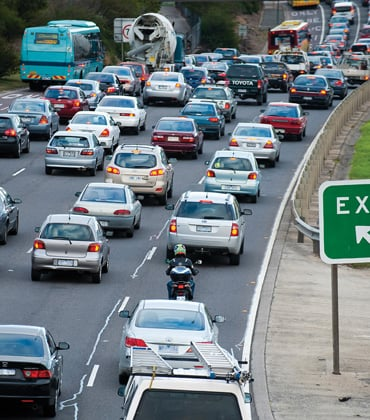
\includegraphics[width=6cm]{Figures/logo}}  %NEW: Changing logo
\def\extraspace{\vspace*{1.6cm}}
\makeatletter
\def\contactdetails{\faicon{phone} & \@telephone \\
                    \faicon{envelope} & \@email}
\makeatother

%%%% FRONT PAGE OF REPORTS

\def\reporttype{Report for}

\long\def\front#1#2#3{
\newpage
\begin{singlespacing}
\thispagestyle{empty}
\vspace*{-1.4cm}
\hspace*{-1.4cm}
\hbox to 16cm{
  \hbox to 6.5cm{\vbox to 14cm{\vbox to 25cm{
    \logo
    \vfill
    \parbox{6.3cm}{\raggedright
      \sf\color[rgb]{0.8, 0.7, 0.1 }    % NEW color 
      {\large\textbf{\name}}\par
      \vspace{.7cm}
      \tabcolsep=0.12cm\sf\small
      \begin{tabular}{@{}ll@{}}\contactdetails
      \end{tabular}
      \vspace*{0.3cm}\par
      ABN: \abn\par
    }
  }\vss}\hss}
  \hspace*{0.2cm}
  \hbox to 1cm{\vbox to 14cm{\rule{4pt}{26.8cm}\vss}\hss\hfill}  %NEW: Thicker line
  \hbox to 10cm{\vbox to 14cm{\vbox to 25cm{   
      \vspace*{3cm}\sf\raggedright
      \parbox{11cm}{\sf\raggedright\baselineskip=1.2cm
         \fontsize{24.88}{30}\color[rgb]{0, 0.29, 0.55}\sf\textbf{#1}}   % NEW: title color blue
      \par
      \vfill
      \large
      \vbox{\parskip=0.8cm #2}\par
      \vspace*{2cm}\par
      \reporttype\\[0.3cm]
      \hbox{#3}%\\[2cm]\
      \vspace*{1cm}
      {\large\sf\textbf{\Date~\Month~\Year}}
   }\vss}
  }}
\end{singlespacing}
\newpage
}

\makeatletter
\def\titlepage{\front{\expandafter{\@title}}{\@author}{\@organization}}
\makeatother

\usepackage{setspace}
\setstretch{1.5}

%% Any special functions or other packages can be loaded here.
\usepackage{booktabs}
\usepackage{longtable}
\usepackage{array}
\usepackage{multirow}
\usepackage{wrapfig}
\usepackage{float}
\usepackage{colortbl}
\usepackage{pdflscape}
\usepackage{tabu}
\usepackage{threeparttable}
\usepackage{threeparttablex}
\usepackage[normalem]{ulem}
\usepackage{makecell}
\usepackage{xcolor}


\begin{document}
\titlepage

\section*{Introduction}

Road safety is a major public policy issue in the state of Victoria. Every year, there are thousands of accidents on the state's road network, in which hundreds of people are killed or injured. The aim of this report is to explore the trends and patterns in Victoria's road safety data, identifying which factors are associated with a higher risk of accident or death, and seeking to explain those relationships.

\subsection*{Data}

The data used in the report was obtained from VicRoads, and contains comprehensive information on approximately 200,000 accidents that occurred in the state from 2006 to 2020. The dataset is licensed with Creative Commons Attribution 4.0 International.

\subsection*{Research questions}

The research questions are as follows:

\begin{enumerate}
\def\labelenumi{\arabic{enumi}.}
\item
  The impact of temporal factors, such as year, weekday and hour, on the number of accidents.
\item
  The relationship of speed and the age of vehicles with the death rate from accidents.
\item
  The effect of age and gender on accident numbers, as well as which roads in Victoria are most accident-prone and most deadly.
\end{enumerate}

\section*{Temporal factors analysis}

\subsection*{Accidents per year}

\begin{figure}
\centering
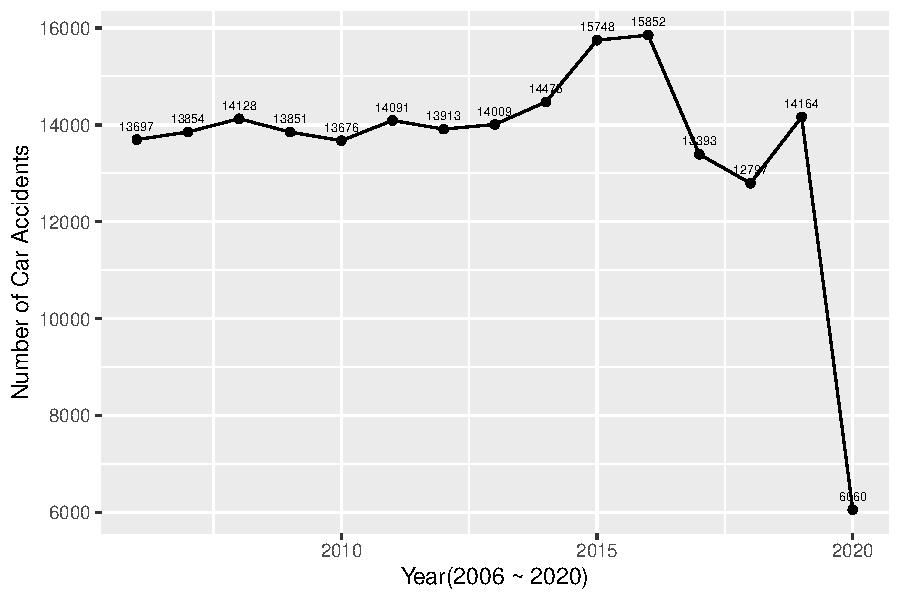
\includegraphics{Report_files/figure-latex/chen1-1.pdf}
\caption{\label{fig:chen1}Car Accidents per year}
\end{figure}

According to plot \ref{fig:chen1}, the increasing number of car accidents remained relatively stable from 2006 to 2014, around 14000. After 2014, the increasing speed became faster and then reached the first peak in 2015, second peak in 2016: 15852.After 2016, it started to drop. There is one outstanding change between 2019 and 2020, which it plummeted down from 14164 to 6060. The possible reason is the coming of covid 19 pandemic and the lockdown of Victoria, which made less car on roads, less accidents happened.

\subsection*{Accidents by weekday}

\begin{table}

\caption{\label{tab:unnamed-chunk-1}Number of Car Accidents happended by weekday}
\centering
\begin{tabular}[t]{l|r}
\hline
Weekday & Accidents\\
\hline
Sunday & 25181\\
\hline
Monday & 27383\\
\hline
Tuesday & 29132\\
\hline
Wednesday & 29939\\
\hline
Thursday & 30950\\
\hline
Friday & 32240\\
\hline
Saturday & 28883\\
\hline
\end{tabular}
\end{table}

\begin{figure}
\centering
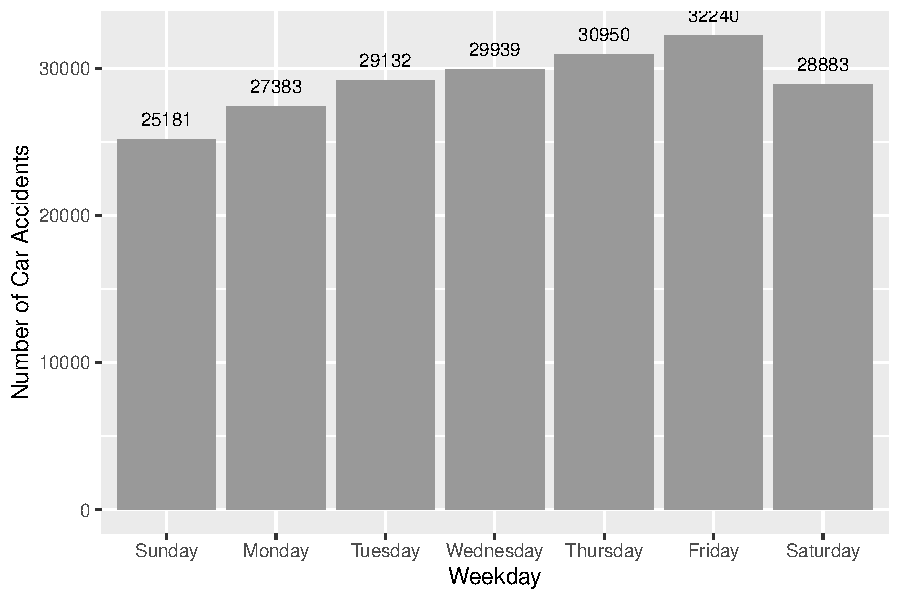
\includegraphics{Report_files/figure-latex/chen2-1.pdf}
\caption{\label{fig:chen2}Car Accidents by weekday}
\end{figure}

Regarding to plot \ref{fig:chen2},it indicates that there is a stable increasing number of car accidents from Sunday to Friday then reach the highest number on Friday. We could understand it from the following reasons: people are getting more and more exhausted during the whole working week, and many people will choose to hang out on Friday night which increase the percentage of driving drunk or reckless.

\subsection*{Accidents by hour and Death Rate by hour}

\begin{figure}
\centering
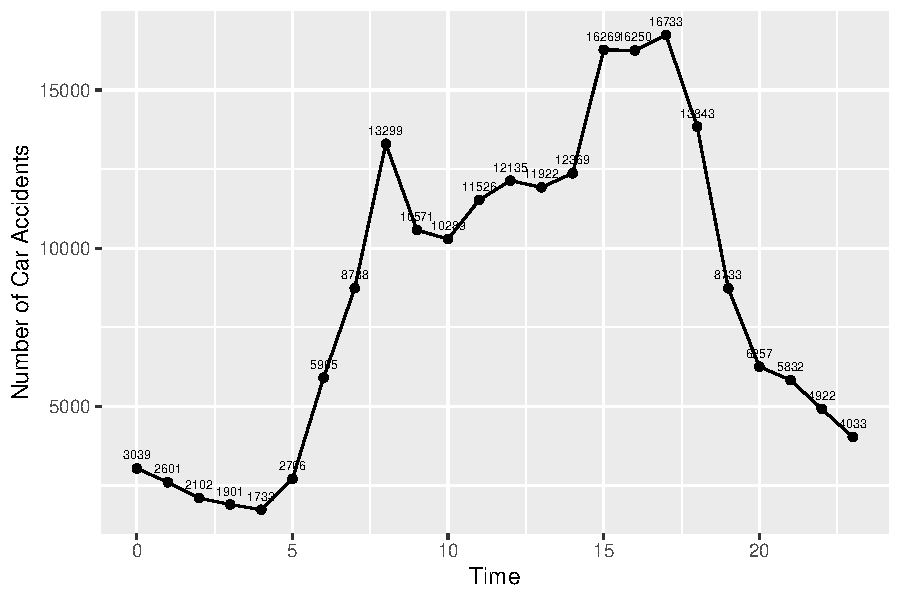
\includegraphics{Report_files/figure-latex/chen3-1.pdf}
\caption{\label{fig:chen3}Car Accidents by hour}
\end{figure}

\begin{figure}
\centering
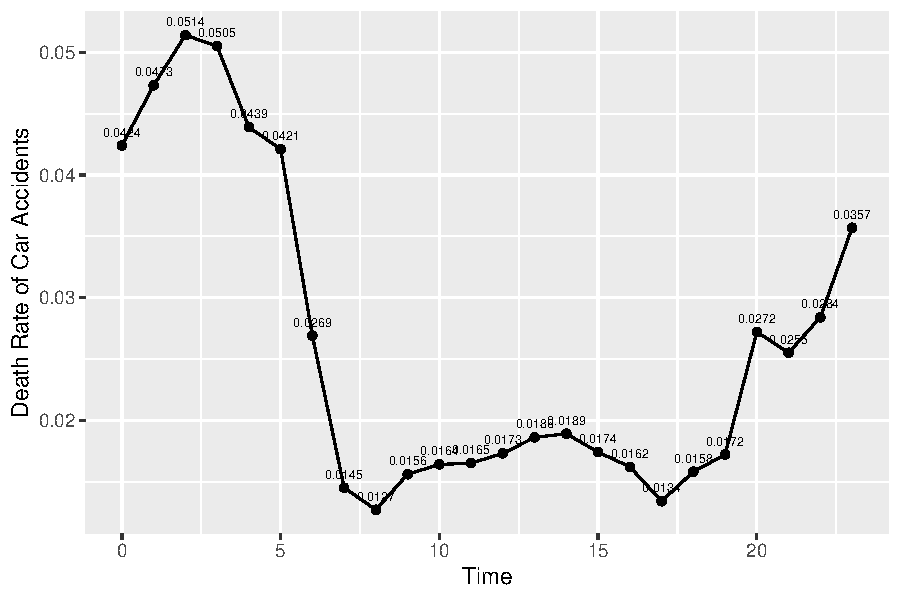
\includegraphics{Report_files/figure-latex/chen4-1.pdf}
\caption{\label{fig:chen4}Death Rate by hour}
\end{figure}

When comparing plot \ref{fig:chen3} and plot \ref{fig:chen4}, we could notice that these two trend are indicating opposite story, which is the higher number of accidents actually with lower death rate during the same specific time. For examle, 8 o'çlock in the morning reached the first peak of car accidents. However, the death rate of it was the lowest. And the point of 5 o'clock tells a similar story. The \ref{fig:chen4} actually shows although 2 o'clock in the midnight has almost the lowest volume of car accidents, it has the highest death rate.

The possible reasons for above results are: both 8 o'clock in the morning and 5 o'clock in the afternoon are the commuter time, which make the traffic busier and more cars on roads, so more accidents. However, most of the accidents won't be too server due to the packed traffic. The 2 o'clock in the midnight is different. First, drivers would be more sleepy and more drivers would take the risk of drunk driving after attending parties in the night which make the accidents have a higher death rate.

\section*{Effect of speed and vehicle age on death rate}

\subsection*{Death rate by speed zone}

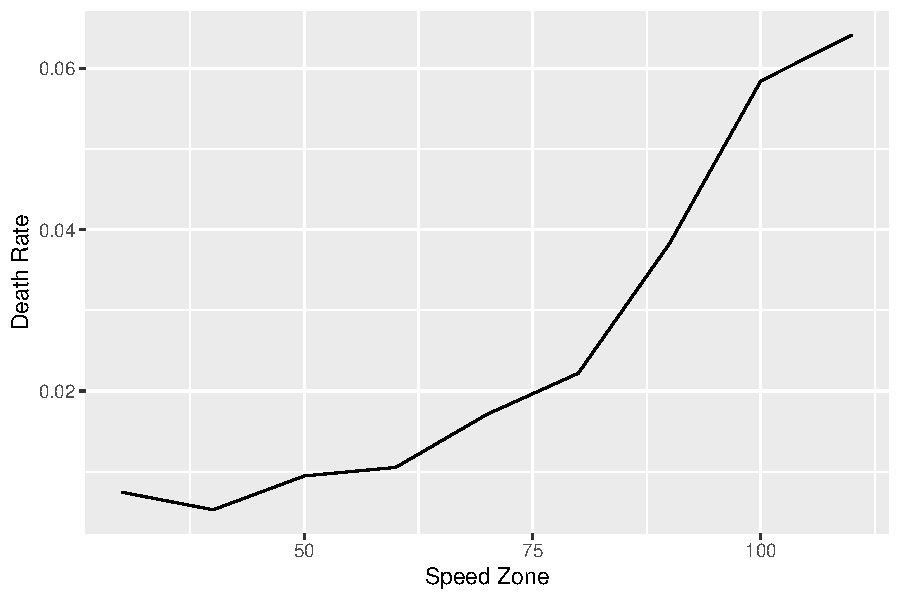
\includegraphics{Report_files/figure-latex/deaths-per-accident-plot-1.pdf}

\begin{table}

\caption{\label{tab:deaths-per-accident-table}Death Rate per Speed Zone}
\centering
\begin{tabular}[t]{l|r|r|r}
\hline
Speed Zone & Accidents & Deaths & Death Rate\\
\hline
030 & 269 & 2 & 0.0074349\\
\hline
040 & 8937 & 47 & 0.0052590\\
\hline
050 & 36149 & 342 & 0.0094608\\
\hline
060 & 69133 & 727 & 0.0105160\\
\hline
070 & 15145 & 259 & 0.0171014\\
\hline
075 & 62 & 2 & 0.0322581\\
\hline
080 & 27794 & 617 & 0.0221990\\
\hline
090 & 940 & 36 & 0.0382979\\
\hline
100 & 31240 & 1827 & 0.0584827\\
\hline
110 & 2151 & 138 & 0.0641562\\
\hline
777 & 249 & 1 & 0.0040161\\
\hline
888 & 930 & 6 & 0.0064516\\
\hline
999 & 10709 & 30 & 0.0028014\\
\hline
\end{tabular}
\end{table}

For this question, the variable Death Rate is defined as the number of deaths in a given speed zone over the time period analysed, divided by the number of accidents. All of these figures can be seen in the table.

The analysis for this question works on the reasonable assumption that accidents that occur in higher speed zones occur at higher speeds. The analysis shows that there is a very strong association between the level of speed permitted in a certain zone, and the likelihood of dying in an accident in that zone. As the level of speed permitted increases, the probability of dying in an accident rises sharply. The death rate from accidents in 40km/h zones is around 0.005, where as in 110km/h zones, the death rate is around 0.064; that is, you are nearly 13 times more likely to be killed in an accident in a 110km/h zone, as opposed to a 40km/h zone.

The reason for this difference in the death rate is fairly obvious; higher speeds contribute greatly to the severity of accidents. A person's car may be lightly to moderately damaged in a low-speed collision, but is much more likely to suffer massive damage in a high speed collision. This in turn drastically increases the risk of serious injury or death for the occupants.

\subsection*{Death rate by year of vehicle manufacture}

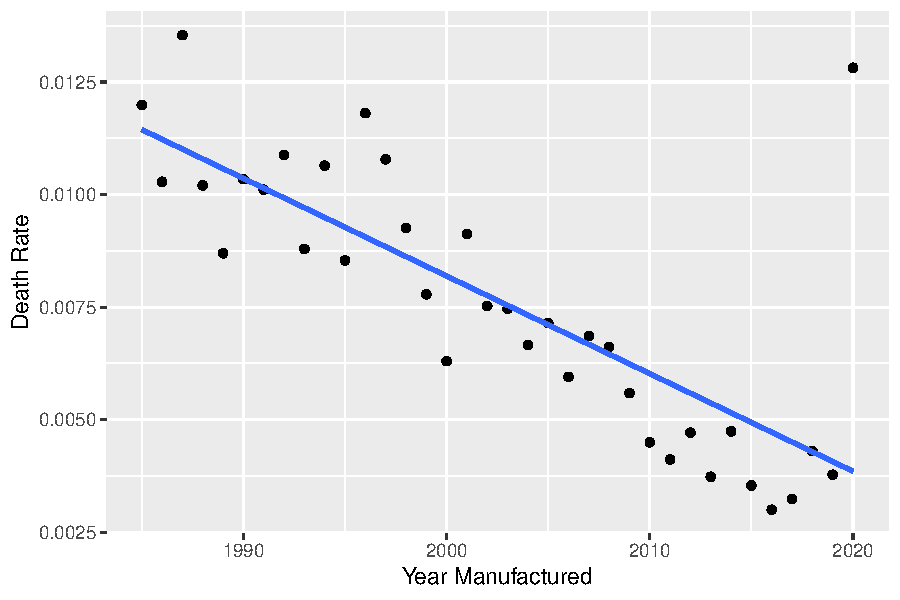
\includegraphics{Report_files/figure-latex/plot-death-rate-by-year-manuf-1.pdf}

\subsubsection*{Regression model residual panel}

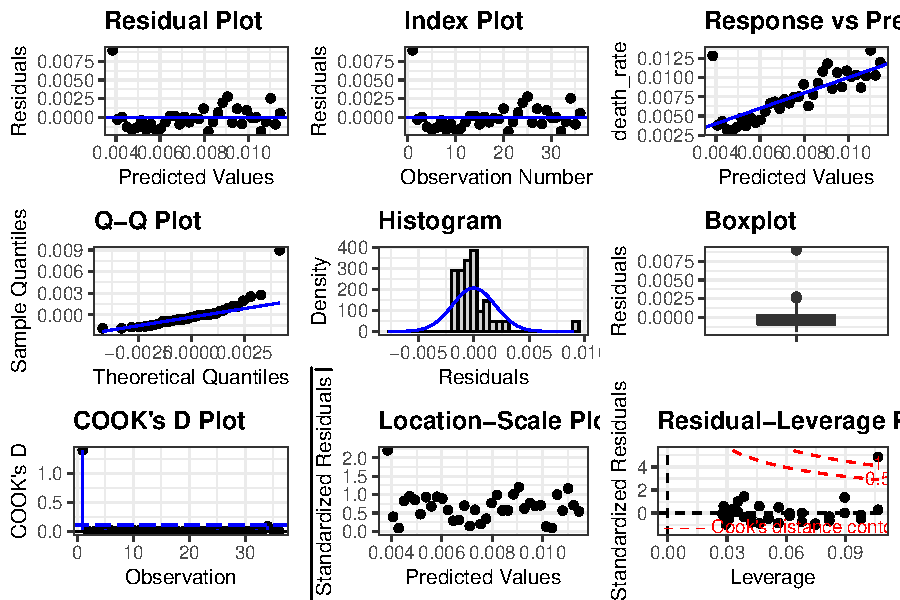
\includegraphics{Report_files/figure-latex/regression-model-1.pdf}

\subsubsection*{Goodness of fit tables}

\begin{table}
\centering
\begin{tabular}{l|r|r|r|r}
\hline
term & estimate & std.error & statistic & p.value\\
\hline
(Intercept) & 0.4420226 & 0.0627854 & 7.040211 & 0e+00\\
\hline
vehicle\_year\_manuf & -0.0002169 & 0.0000314 & -6.918470 & 1e-07\\
\hline
\end{tabular}
\end{table}

\begin{table}
\centering
\begin{tabular}{r|r|r|r|r|r|r|r|r|r|r|r}
\hline
r.squared & adj.r.squared & sigma & statistic & p.value & df & logLik & AIC & BIC & deviance & df.residual & nobs\\
\hline
0.5846833 & 0.5724681 & 0.0019542 & 47.86523 & 1e-07 & 1 & 174.5064 & -343.0127 & -338.2622 & 0.0001298 & 34 & 36\\
\hline
\end{tabular}
\end{table}

For this question, the variable Death Rate is defined as the number of deaths in accidents involving cars from a particular year of manufacture, divided by the number of accidents.

The analysis of the death rate by year of vehicle manufacture shows that there is a relatively strong negative correlation between the recentness of the year of manufacture of a vehicle, and the likelihood that a vehicle manufactured in that year will be involved in a fatal accident. The graph shows that a person is more than twice as likely to be killed in an accident if they are in a car manufactured in the late 1980s, as opposed to a car manufactured in the last 5 years.

In the linear model which was fitted to the data, for every year older a car is, the death rate increases by around 0.0002 deaths per accident. This linear model fits the data quite well; the R-squared is around 0.6, and the residuals are fairly evenly spaced around 0.

The reason for the decline in the death rate associated with more recently manufactured vehicles is improved safety standards. Cars built today contain far more structural features designed to protect occupants in the event of an accident. They also possess better braking capability, as well as extensive electronic systems that warn drivers of impending hazards.

\section*{Accidents by Locations, Gender and Road User Type}

\subsection*{Accidents Map}

\begin{figure}
\centering
\includegraphics{Report_files/figure-latex/accidents-map-1.pdf}
\caption{\label{fig:accidents-map}Map of accident locations in Victoria}
\end{figure}

As shown in figure \ref{fig:accidents-map}, accidents are most highly concentrated around metropolitan Melbourne, and gradually reduce in volume the further we move from Melbourne, with pockets of concentrations in the regional cities such as Bendigo, Ballarat and Geelong. This is due to the population being most present in metropolitan Melbourne, resulting in more accidents, and the population declining as we drift away, resulting in less accidents.

\subsection*{Roads with Most Accidents and Highest Death Rates}

\begin{table}

\caption{\label{tab:accidents-by-road}Accidents by road}
\centering
\begin{tabular}[t]{l|r}
\hline
Road & Accidents\\
\hline
PRINCES HIGHWAY & 3581\\
\hline
HIGH STREET & 3096\\
\hline
NEPEAN HIGHWAY & 2376\\
\hline
SPRINGVALE ROAD & 1663\\
\hline
SOUTH GIPPSLAND HIGHWAY & 1538\\
\hline
SYDNEY ROAD & 1538\\
\hline
MONASH FREEWAY & 1533\\
\hline
MAROONDAH HIGHWAY & 1335\\
\hline
\end{tabular}
\end{table}

\begin{table}

\caption{\label{tab:deadliest-road}Deadliest roads}
\centering
\begin{tabular}[t]{l|r|r|r}
\hline
Road & Accidents & Deaths & Deaths\_per\_accident\\
\hline
GLENELG HIGHWAY & 231 & 28 & 0.1212121\\
\hline
GOULBURN VALLEY HIGHWAY & 344 & 39 & 0.1133721\\
\hline
WIMMERA HIGHWAY & 156 & 17 & 0.1089744\\
\hline
MURRAY VALLEY HIGHWAY & 727 & 76 & 0.1045392\\
\hline
STRZELECKI HIGHWAY & 106 & 11 & 0.1037736\\
\hline
HAMILTON HIGHWAY & 223 & 21 & 0.0941704\\
\hline
MELBA HIGHWAY & 211 & 18 & 0.0853081\\
\hline
NORTHERN HIGHWAY & 300 & 25 & 0.0833333\\
\hline
\end{tabular}
\end{table}

According to table \ref{tab:accidents-by-road}, \textbf{Princes Highway}, \textbf{High Street} and \textbf{Nepean Highway} are the three most accident prone roads in Victoria with 3581, 3096, 2376 accidents, respectively. It is important to note that roads with the name ``High Street'' are quite common and are present in various suburbs in Victoria, therefore the ``High Street'' displayed in the table is likely a combination of all the accidents that occurred in all the High Streets. When examining the deadliest roads from table \ref{tab:deadliest-road}, it is immediately apparent that \textbf{Highways} are the deadliest type of road in Victoria, this is likely a result of highways being locations of higher speed zones, which as we have seen from the previous section, lead to higher death rates.

\subsection*{Accidents by Gender}

\begin{table}

\caption{\label{tab:accidents-gender-table}Number of accidents by gender}
\centering
\begin{tabular}[t]{l|r}
\hline
Sex & Accidents\\
\hline
Male & 171043\\
\hline
Female & 118307\\
\hline
Unknown & 8831\\
\hline
\end{tabular}
\end{table}

\begin{figure}
\centering
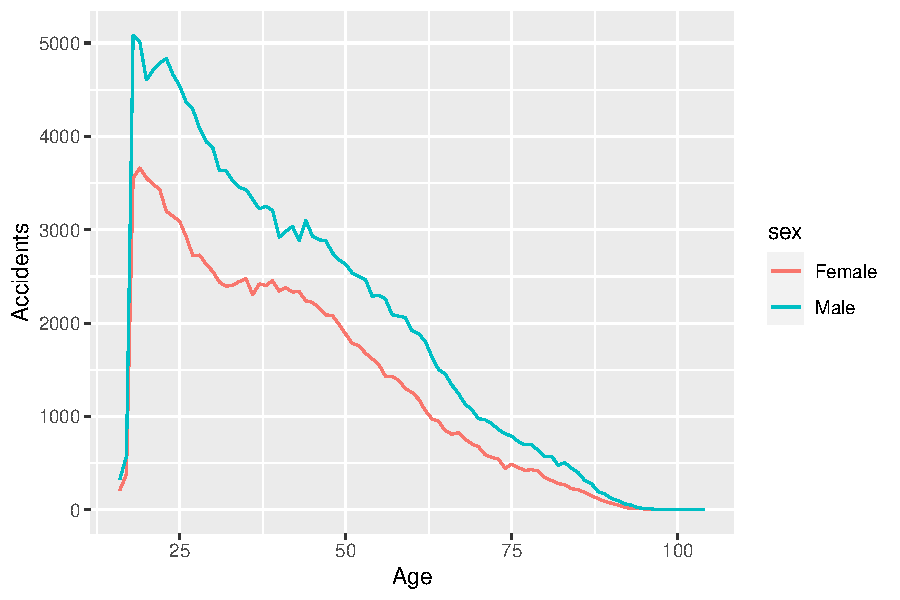
\includegraphics{Report_files/figure-latex/accidents-gender-plot-1.pdf}
\caption{\label{fig:accidents-gender-plot}Number of accidents by gender and age}
\end{figure}

Table \ref{tab:accidents-gender-table} shows that there are more accidents committed by males (171,043) than by females (118,307). Figure \ref{fig:accidents-gender-plot} extends that differential by showing that males commit more accidents than females at all age groups. This could be a result of larger male presence on the roads than females, for example the majority of truck drivers and taxi/uber drivers are male, therefore representing higher numbers and longer times spent on the road. What is common between both genders, however, is that the accident numbers are highest for young and inexperienced drivers before steadily declining as age and experience increase. This is consistent with the findings from \textcite{gislason1997medical}.

\subsection*{User Type Death Rates}

\begin{figure}
\centering
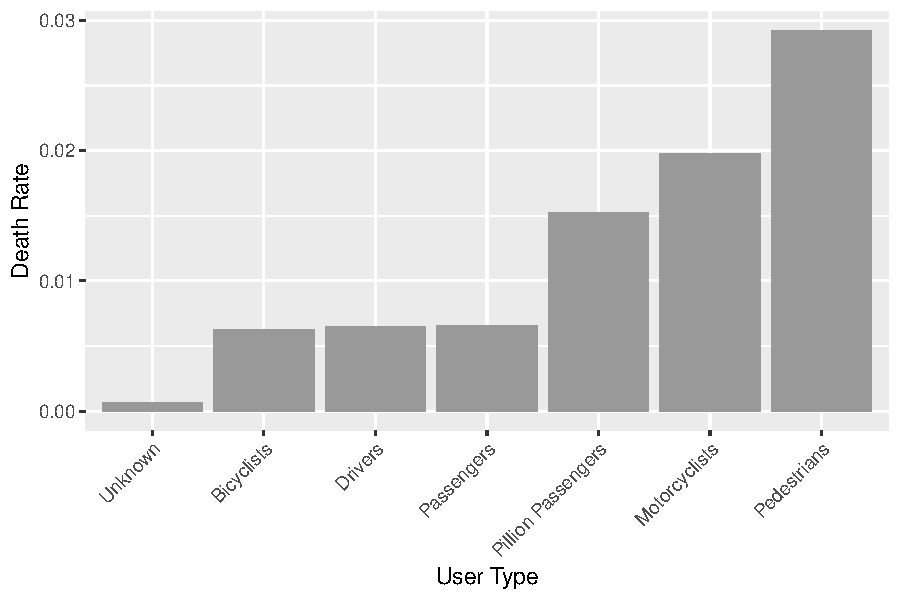
\includegraphics{Report_files/figure-latex/user-death-rate-1.pdf}
\caption{\label{fig:user-death-rate}Death rate by road user type}
\end{figure}

As per figure \ref{fig:user-death-rate}, \textbf{pedestrians} are at the most risk of death per accident, this is expected as pedestrians have no protection at all. \textbf{Motorcyclists} and \textbf{pillion passengers} (motorcycle passengers) occupy the second and third highest death rate per accident. It is surprising, however, that \textbf{bicyclists}'s death rate is similar to that of car drivers and passengers, as one would expect that bicyclists would have a death rate similar to that of pedestrians or motorcyclists, due to the lack of protection besides a helmet.

\section*{Conclusions}

The analysis produced several pieces of informative results. First, it was found that accidents increase gradually throughout the working week, and that whilst accidents are most common in evening peak hour, that period is the least deadly time of day in which to have an accident. Higher speeds dramatically increase the risk of death in an accident, and more recent car models are far less prone to fatal accidents than older varieties. Finally, being young and male is most strongly associated with having an accident, and regional highways tend to be the deadliest roads in the state.

\section*{Software and Packages}

This report was created using \textcite{Rcore}. We also used packages created by \textcite{ggresidpanel}, \textcite{broom}, \textcite{tidyverse}, \textcite{lubridate}, \textcite{janitor}, \textcite{knitr}, \textcite{kableextra}, \textcite{bookdown}, \textcite{ggmap}, \textcite{ggthemes}.

\printbibliography

\end{document}
